\section{Slew Rate}
In diesem Versuch soll die Slow-rate eines Operationsverst\"arker bestimmt werden.
\subsection{Experimentelle Durchf\"urung}
Zur Messung der Slow-rate wird erneut die Schaltung aus Abbildung 1 verwendet. Bei diesem Versuch wird allerdings die Betriebspannung konstant bei U$_{\text{DD}}$ $=$ 12~$V$ gehalten. Au\ss erdem wird am Eingang U$_e$ ein Funktionsgenerator mit Rechtecksignal angeschlossen(V$_{\text{pp}}$~$=$~5~$V$ und f $=$ 1~$kHz$). Die Ausgangsspannung wird mit Hilfe eines Oszilloskop gemessen. Die Steigung der Kennlinie, die daraus resultiert, entspricht der Slow-rate. \\
Die Slow-rate kann mit folgende Formel bestimmen:
\begin{equation*}
SR = \frac{\Delta U}{\Delta t}
\end{equation*}
Zum Schluss dieses Teil Versuches sollte die Ausgangsspannung bei drei verschiedene Frequenzen: 20~$kHz$, 200~$kHz$ und 2000~$kHz$ mit einem Sinus als Eingangsignal bestimmt werden.
\subsection{Ergebnisse und Diskussion}
Aus Abbildung 2 lassen sich folgende Werte ablesen, mit dennen man die Slow-rate bestimmen kann: $\Delta t$~$=$~180~$ns$ und $\Delta U$~$=$~2,36~$V$. 
\begin{equation*}
SR = \frac{2,36}{180} = 13,11~V/\mu s
\end{equation*}
In Datenblatt ist eine Slow-rate von SR$_{\text{typ}}$ $=$ 13~$V/\mu s$. Unser ermittelter Wert kommt dieser Slow-rate sehr nah. 
\begin{figure}[!ht]
\begin{center}
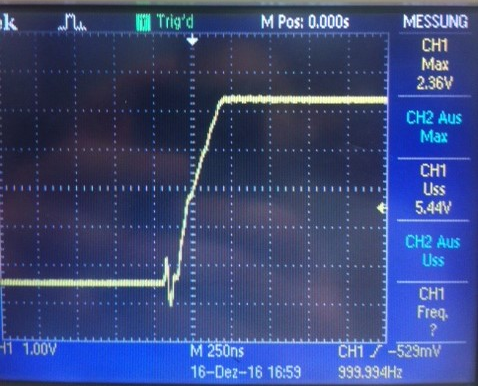
\includegraphics[scale=0.6]{bild/slow-rate}
\caption{Kurve der slow-rate Messung}
\end{center}
\end{figure}
Es zeigt sich, dass der Spannungsfolger eine konstante Amplitude bei ca. 5~$V_{\text{pp}}$  bei den Frequenzen 20~$kHz$ und 200~$kHz$ besitzt(Abbildung 3, 4). Bei relativ hohen Frequenzen in unserem Fall 2000~$kHz$ ver\"andert sich das Sinussignal sehr stark(Abbildung 5). Das Ausgangssignal hat eine geringere Amplitude (3.60~$V$) und die Kurve ist nicht mehr rund, sondern eckig. Der Grund hierf\"ur ist, dass der Verst\"arker bei zu hohen Frequenzen dem Signal nicht mehr folgen kann, was auf die interne Kapzit\"at des Verst\"arker zur\"uck zuf\"uhren ist.
\begin{figure}[!ht]
\begin{center}
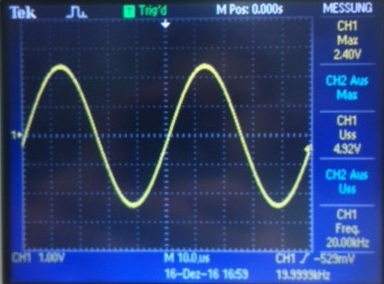
\includegraphics[scale=0.8]{bild/image1}
\caption{Frequenzverhalten des OPs bei $10kHz$}
\end{center}
\end{figure}
\begin{figure}
\end{figure}
\begin{figure}[!ht]
\begin{minipage}{0.4\textwidth}
\begin{center}
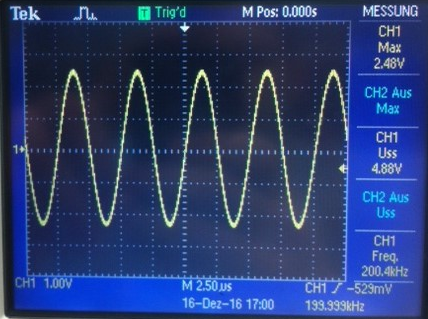
\includegraphics[scale=0.6]{bild/image2}
\caption{Frequenzverhalten des OPs bei $100kHz$}
\end{center}
\end{minipage} \hfill
\begin{minipage}{0.4\textwidth}
\begin{center}
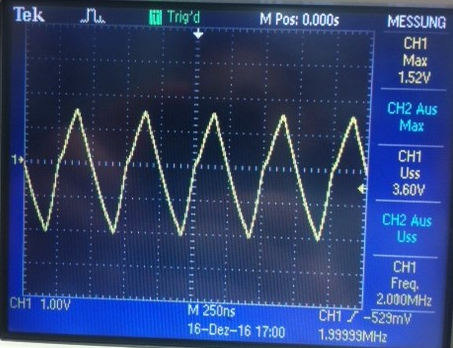
\includegraphics[scale=0.6]{bild/image3}
\caption{Frequenzverhalten des OPs bei $1000kHz$}
\end{center}
\end{minipage}
\end{figure}
